Typically observers can measure only the period and a few derivatives from a
pulsar (the method to do this is described in section \ref{sec: pulsar timing
methods}).  We now consider what can be learnt from the observed $P$ and
$\Pdot$ if we assume a simple dipole spindown model. In figure \ref{fig:
DipoleSpindownSimple} we illustrate a rotating rigid body with a dipole fixed
at an angle $\alpha$ to the rotation axis; we will assume the body rotates in
vacuum. 

\begin{figure}[htb]
    \centering
    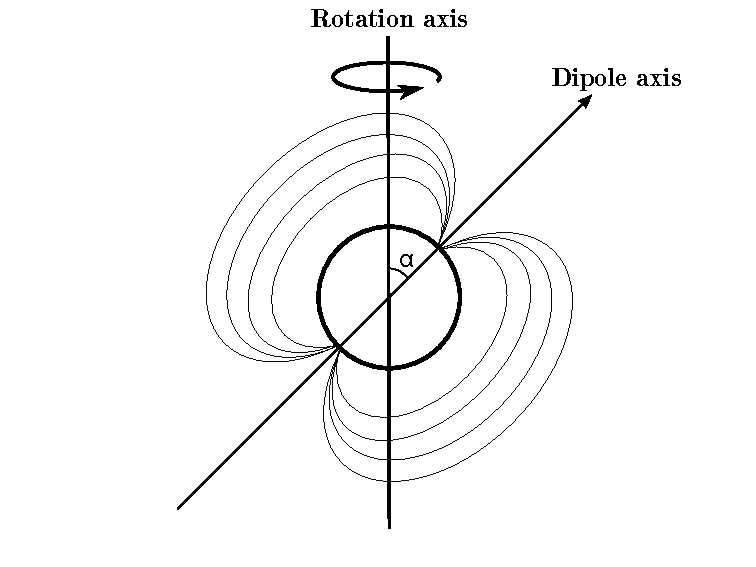
\includegraphics[width=.5\textwidth]{DipoleModelSimple}
    \caption{An illustration of the dipole spindown model. The dipole and some 
    of the closed field lines are fixed at an angle $\alpha$ to the rotation 
    axis. As the body rotates, radiation is emitted along both ends of the dipole
    axis producing a torque on the body.}
    \label{fig: DipoleSpindownSimple}
\end{figure}

The rotational energy of a body spinning at $\Omega$ with a moment of inertia
$I_{0}$ is given by
\begin{equation}
    E = \frac{1}{2}I_{0}\Omega^{2}.
\end{equation}
Differentiating this expression, we equate this loss of rotational energy
to the rate at which a magnetic dipole in free space radiates energy as found
by \citet{Pacini1967}:
\begin{equation}
    I_{0}\Omega\dot{\Omega} = 
                    -\frac{2\Omega^{4}}{3 c^{3}} R^{6} B_{0}^{2}\sin^{2}\alpha,
    \label{eqn: equate dKE to dEM} 
\end{equation}
where $R$ is the radius of the NS, $B_{0}$ is the surface magnetic field, and
$\alpha$ is the angle between the dipole and the rotation axis.  

In this simple model we can interpret the type of spindown by defining a power
law dependence for the braking
\begin{equation}
    \dot{\Omega} = -k \Omega^{n},
    \label{eqn: power law spindown}
\end{equation}
where $k$ is constant of proportionality, $\dot{\Omega}$ is the spindown, and
$n$ defines the \emph{braking index}. Rearranging equation 
\eqref{eqn: equate dKE to dEM} to compare with this power law, we find that for
magnetic dipole spindown:
\begin{align}
    n = 3 && \textrm{ and } && k = \frac{2B_{0}^{2}R^{6} \sin^{2}\alpha}{3 c^{3} I_{0}}.
    \label{eqn: n and k}
\end{align}
\textcolor{red}{This is different to Shapiro by a factor of 1/4}\\
For gravitational wave powered spindown, it can be shown that $n=5$
(see \citet{Shapiro83}). This suggests a powerful method to determine the spindown
mechanism if the braking index can be measured. This can be done if
$\ddot{\Omega}$ can be measured: rearranging equation \eqref{eqn: power law
spindown} to give
\begin{equation}
    n = \frac{\ddot{\Omega}\Omega}{\dot{\Omega}^{2}}.
    \label{eqn: measured braking index}
\end{equation}
The results of this are are discussed further in section \ref{sec: evidence from
    anomalous braking indices}.

For a pulsar powered by rotation, equation \eqref{eqn: power law spindown} can
be integrated between the initial values ($t=0, \Omega=\Omega_{i}$) and the
observed value ($\Omega_{o}$) to give an expression for the age of the pulsar
\begin{equation}
    t = \frac{1}{(1-n)} \frac{\Omega_{o}}{\dot\Omega_{o}} 
        \left(1 - \frac{\Omega_{o}^{n-1}}{\Omega_{i}^{n-1}}\right).
\label{eqn: characteristic age}
\end{equation}
Assuming magnetic dipole braking ($n=3$) and $\Omega_{i} \gg \Omega_{o}$ we can
approximate to a characteristic age 
\begin{equation}
    \tau = \frac{-1}{2}\frac{\Omega_{\textrm{o}}}{\dot\Omega_{o}}
         = \frac{1}{2}\frac{P}{\Pdot}.
\end{equation}
Where $P=\frac{2\pi}{\Omega}$ is the pulse period and
$\dot{P}=-2\pi\frac{\dot{\Omega}}{\Omega^{2}}$ is the period derivative.
Similarly
rearranging equations \eqref{eqn: power law spindown} and 
\eqref{eqn: n and k} we can estimate the surface magnetic field strength by
\begin{equation}
    B_{0} = \left(\frac{3 c^{3} I_{0}}{2R^{6} \sin^{2}\alpha}\right)^{\frac{1}{2}} 
            \left(\frac{-\dot{\Omega}}{\Omega^{3}}\right)^{\frac{1}{2}}
          = \frac{1}{2\pi}\left(\frac{3 c^{3} I_{0}}{2R^{6} \sin^{2}\alpha}\right)^{\frac{1}{2}}
           \sqrt{P \Pdot}
\label{eqn: surface magnetic field}
\end{equation}
In general we do not know the inclination angle $\alpha$, but we can evaluate a 
minimum magnetic field strength by setting $\alpha=\pi/2$. In CGS units for a
canonical pulsar with $R=10^{6}$~cm, $I_{0}=10^{45}$~g~cm$^{2}$ we can approximate
the magnetic field strength as
\begin{equation}
    B_{0} = 3.2 \times 10^{19} \sqrt{P \Pdot}.
\label{eqn: surface magnetic field canonical}
\end{equation}


